\documentclass{ieeeaccess}
\usepackage{cite}
\usepackage{amsmath,amssymb,amsfonts,amsthm}
\usepackage{mathtools}
\usepackage{graphicx}
\graphicspath{{../figures/}}
\usepackage{textcomp}
\usepackage[utf8]{inputenc}
\usepackage[T1]{fontenc}
\usepackage{bm}
\usepackage{booktabs}
\usepackage{xcolor}
\usepackage{hyperref}
\usepackage{multirow}
\usepackage{array}
\usepackage{tabularx}
\usepackage{enumitem}
\usepackage{siunitx}

\makeatletter
\AtBeginDocument{\DeclareMathVersion{bold}
\SetSymbolFont{operators}{bold}{T1}{times}{b}{n}
\SetSymbolFont{NewLetters}{bold}{T1}{times}{b}{it}
\SetMathAlphabet{\mathrm}{bold}{T1}{times}{b}{n}
\SetMathAlphabet{\mathit}{bold}{T1}{times}{b}{it}
\SetMathAlphabet{\mathbf}{bold}{T1}{times}{b}{n}
\SetMathAlphabet{\mathtt}{bold}{OT1}{pcr}{b}{n}
\SetSymbolFont{symbols}{bold}{OMS}{cmsy}{b}{n}
\renewcommand\boldmath{\@nomath\boldmath\mathversion{bold}}}
\makeatother

\newtheorem{proposition}{Proposition}
\newtheorem{problem}{Problem}
\newtheorem{remark}{Remark}

\newcommand{\R}{\mathbb{R}}
\newcommand{\norm}[1]{\left\| #1 \right\|}
\newcommand{\Jv}{\bm{J}_{\!v}}
\newcommand{\Jw}{\bm{J}_{\!\omega}}
\newcommand{\Jfull}{\bm{J}}
\newcommand{\Pobs}{\bm{P}}
\newcommand{\Pff}{\bm{P}_{\!f\!f}}
\newcommand{\SEthree}{\mathrm{SE}(3)}
\newcommand{\tauext}{\bm{\tau}_{\mathrm{ext}}}
\newcommand{\tauact}{\bm{\tau}_{\mathrm{act}}}

\begin{document}
\history{Date of publication xxxx 00, 0000, date of current version xxxx 00, 0000.}
\doi{10.1109/ACCESS.2026.0000000}

\title{Sensorless Contact-Force Estimation on Low-DoF, Velocity-Actuated
Manipulators: A Quantitative Design Framework}

% ⚠️ AFILIACION: se conserva la primera (LASER/UFPB), que es la que corresponde al
% correo institucional del autor. Si la institucion de origen es otra, cambiar
% aqui. Las afiliaciones heredadas del otro trabajo se eliminaron.
\author{{Bryan S. Guevara}\authorrefmark{1}}

\address[1]{Laboratory of Systems and Robotics Engineering (LASER),
Center of Informatics (CI), Federal University of Para\'iba (UFPB),
Jo\~ao Pessoa, PB 58051-900, Brazil
(e-mail: bryansgue@laser.ci.ufpb.br)}

\markboth
{B. S. Guevara:~Sensorless Contact-Force Estimation on Low-DoF Arms}
{B. S. Guevara:~Sensorless Contact-Force Estimation on Low-DoF Arms}

\begin{abstract}
Compliant physical interaction on low-cost manipulators must work without a
force/torque sensor, whose price exceeds that of the arm, and with servos
commanded in velocity rather than torque. That a residual observer cannot resolve
a full wrench from fewer than six joints, and that a point-contact model reduces
the unknown to three dimensions, is established. It does not say how much force
is lost, in which directions, or at which postures. This paper supplies that
quantification. The force block of the wrench projector predicts the directional
structure of the error: over $12\,000$ push directions the loss is a linear
function of the alignment with the least observable direction, at correlation
$0.9993$. Over $2197$ configurations of a 4-DoF arm the six-dimensional inversion
discards $50.5\,\%$ of an applied unit force on average and up to $99.6\,\%$,
while still correlating with ground truth at $0.997$, so a validation that looks
convincing can hide a large gain error.
Rejecting postures below $\sigma_{\min}(\bm J_{\!v})=0.06$ halves the
ninetieth-percentile error of the point-contact estimator and leaves the
six-dimensional error untouched, separating amplified noise from structural
misattribution. Velocity-level actuation, usually regarded as an obstacle,
instead confines the dynamic model to the estimator: the residual is invariant to
the inner servo loop, whose gain therefore need not be identified, and a
kinematic controller reproduces the compliant behavior at one twenty-fifth of the
cost. All results are obtained in simulation against a model agreeing with an
independent physics engine to $10^{-10}$; the hardware experiment that would test
the directional prediction and the conditioning law is specified but not run.
\end{abstract}

\begin{keywords}
Compliant control, force estimation, low-cost robotics, model
predictive control, physical human-robot interaction, sensorless sensing,
velocity control.
\end{keywords}

\titlepgskip=-21pt

\maketitle

% =========================================================================
\section{Introduction}
\label{sec:introduction}
% =========================================================================

\PARstart{C}{ompliant} physical interaction, in which a manipulator yields to an
external push and recovers its task once released, underpins hand guiding,
contact-rich assembly, and safe operation in shared workspaces. The canonical
implementation measures the interaction wrench with a wrist force/torque (F/T)
sensor and closes an impedance or admittance law around
it~\cite{hogan1985impedance,siciliano1999forcecontrol}.

On research-grade manipulators this is unremarkable. On arms assembled from
commercial smart servos, a class that increasingly serves education, small-scale
automation, and mobile manipulation research, it is not viable. A six-axis F/T
sensor typically costs more than the entire mechanism, and mounting one consumes
payload and structural stiffness that a lightweight arm cannot spare. The economic
argument that motivates a low-cost arm is precisely the argument against
instrumenting it.

The question this paper addresses is therefore a design question rather than a
feasibility one: given a low-DoF arm driven by velocity-controlled smart servos,
what contact force is identifiable, with what accuracy, and how can it be used for
compliant interaction?

\subsection{What is known, and what a designer still cannot compute}
The established sensorless alternative is a momentum or residual observer, which
compares measured joint accelerations and actuator torques against a dynamic model
and attributes the mismatch to an external
wrench~\cite{deluca2005sensorless,deluca2006collision,magrini2014virtual}. The
approach is mature and requires no hardware beyond what a servo already reports;
\cite{haddadin2017survey} surveys its detection, isolation, and identification
variants.

The residual lives in joint space and is mapped to a Cartesian wrench through the
transpose Jacobian pseudoinverse. This step recovers six unknowns from $n$
measurements. That it therefore requires $n\ge6$, and that restricting the unknown
to a force at a known point reduces the task dimension to three, is stated
explicitly by Magrini \emph{et al.}~\cite{magrini2014virtual}, who also demonstrate
on a seven-joint arm that attempting the six-dimensional inversion from too few
informative residual components returns a wrong force together with a moment that
should be zero. The dimensional argument is not in dispute and is not claimed here.

What that argument does not supply is anything a designer can act on. It does not
say how much force is lost, and the answer is not a single number: it depends on
posture and on the direction of the push, and the deficit reappears as a spurious
moment rather than as a visible failure. At the task configuration
$\bm q=[0,\,1.2,\,-0.9,\,0.4]$~rad of the arm studied here, a $6$~N push normal to
the plane of the arm is returned by the six-dimensional inversion as $0.264$~N of
force and $1.230\,\mathrm{N}\cdot\mathrm{m}$ of moment: $96\,\%$ of the force is
reassigned. Two force directions at that same posture pass through unaltered. A
statement about ranks cannot distinguish these cases. Nor is the arm the
limitation: the same push produces $1.2867\,\mathrm{N}\cdot\mathrm{m}$ at the base
joint, so the information is present in the measurement and the estimator discards
it.

The failure is also silent. Section~\ref{sec:res-estimation} reports a compliant loop in
which the six-dimensional estimate tracks the true force at correlation $0.997$
while carrying a $2.227$~N error, because correlation measures shape and the
misattribution is a gain error. A validation that would ordinarily be accepted
therefore certifies an estimator that is wrong by a factor of six.

\subsection{The actuator takes velocity, not torque}
The second half of the design question is the actuator. Smart servos of this class
are commanded in velocity, and the residual observer is formulated in torque. The
apparent mismatch is often taken to mean that sensorless estimation is unavailable
on such hardware, or that the servo loop must first be identified.

Neither is the case, and the reason is that the servo exposes a third signal
besides position and velocity: the effort it is applying, reported as motor
current. That channel is the quantity the residual requires, and it takes the place
of the force/torque sensor throughout this work. Since the residual consumes the
applied torque as measured rather than as modeled, the internal velocity loop may
remain a black box.

Section~\ref{sec:velocity} works out what this changes for the chain from motor
current to commanded joint velocity, and the consequences run in the favorable
direction: the interaction signal migrates from the acceleration to the actuator
torque, the dynamic model is confined to the estimator, and the actuator saturates
below the force range of manual guidance, so the arm yields physically without any
control effort.

\subsection{Contributions}
\label{sec:claims}
As shown in Table~\ref{tab:gap}, residual-based interaction sensing has been
developed for torque-actuated manipulators with six or more joints, where the
wrench inversion is over-determined and the actuator accepts the quantity the
controller computes. Neither condition holds on a low-cost smart-servo arm. This
paper contributes a quantitative design framework for that regime, resting on two
components of unequal weight.

\begin{table}[!t]
\caption{Residual-based interaction sensing: operating regime of representative
approaches.}
\label{tab:gap}
\centering
\footnotesize
\setlength{\tabcolsep}{3pt}
\begin{tabular}{lcccc}
\toprule
 & joints & actuation & inversion & force error\\
\midrule
\cite{deluca2005sensorless}  & $\ge6$ & torque & six-dimensional & --- \\
\cite{deluca2006collision}   & $7$    & torque & six-dimensional & --- \\
\cite{magrini2014virtual}    & $7$    & torque & point contact   & hardware, one pose \\
\cite{haddadin2017survey}    & $\ge6$ & torque & six-dimensional & --- \\
\midrule
this work & $\bm{4}$ & \textbf{velocity} & point contact & over workspace\\
\bottomrule
\end{tabular}
\end{table}

\begin{itemize}[leftmargin=*]
\item \textbf{A quantitative and geometric characterization of the inversion under
a known contact model.} The governing object is $\Pff$, the force block of the
wrench projector. Its spectrum \emph{predicts} the directional structure of the
error rather than merely describing it: sweeping the full sphere of push
directions at six configurations, the loss is a linear function of the alignment
with the least observable eigendirection at correlation $0.9993$ over all
$12\,000$ directions. The workspace sweep then supplies magnitude and prevalence,
$50.5\,\%$ of an applied unit force discarded on average over $2197$
configurations and up to $99.6\,\%$; $\sigma_{\min}(\Jv)$ converts the analysis
into an operating criterion; and the correlation study shows why an apparently
sound validation can conceal a large gain error, at $0.997$ against a $2.227$~N
error. Against an independent physics engine the corrected inversion reduces force
RMSE by a factor of fourteen.

\item \textbf{An estimation and compliance architecture for low-DoF arms actuated
in velocity.} The claim is the whole chain from servo current to commanded joint
velocity, $i\rightarrow\tauact\rightarrow\tauext\rightarrow\hat{\bm f}\rightarrow
\dot{\bm q}_{\mathrm{cmd}}$, and what it removes from the identification burden.
Because the applied torque is measured rather than modeled, the inner velocity
loop does not appear in the reconstruction and its gain never needs to be
identified; the finite-differenced acceleration carries $0.006\,\%$ of the signal
in this regime; the dynamic model is therefore confined to the observer, and a
kinematic controller using neither inertia matrix, bias term, nor servo gain
reproduces the compliant behavior at one twenty-fifth of the cost. What must be
identified on hardware reduces to the mass properties and one torque constant,
both serving estimation only. The architecture is then exercised under a servo
noise model covering current quantization, Coulomb stiction, and encoder
resolution, where the point-contact inversion attains $18.0\,\%$ median relative
error against $69.6\,\%$ over $2000$ randomized trials.
\end{itemize}

The predictive controller of Section~\ref{sec:control} is an integration
demonstrator, not an independent contribution: it shows that the estimate closes a
compliant loop under the constraints of the platform, and its formulation is
standard.

We claim neither of the two ingredients that are individually established. That
$\Jfull^{\!\top}\bm F=\tauext$ requires $n\ge6$ and that restricting the unknown
to a force at a known contact point reduces the task dimension to three are both
stated in~\cite{magrini2014virtual}. What is contributed is the quantification
that turns those statements into design criteria, and the velocity-actuated
regime, which that literature does not address.

The $50.5\,\%$ figure is not itself a general result: it belongs to this arm, this
workspace, and this distribution of push directions. It carries weight because
$\Pff$ explains and predicts it, and the same construction can be evaluated for
any other arm before one is built.

\subsection{Scope and organization}
All results reported here are obtained in simulation, against a model agreeing to
$10^{-10}$ with an independent physics engine that also serves as the plant for the
interaction experiments. Hardware validation is not claimed, and the accuracy
claims should be read as conditional on it: the quantities most likely to degrade
are precisely those the simulator cannot reproduce, namely motor current as a proxy
for applied torque, gearbox friction and stiction, backlash, and the calibration of
the torque constant. Section~\ref{sec:discussion} states the limitations and
specifies the experiment that would settle them. Section~\ref{sec:related}
positions the work,
Section~\ref{sec:system} describes the platform and model,
Sections~\ref{sec:estimation} to~\ref{sec:control} develop the method,
Section~\ref{sec:results} reports experiments, and Section~\ref{sec:conclusion}
concludes.

% =========================================================================
\section{Related Work}
\label{sec:related}
% =========================================================================

\subsection{Sensorless interaction sensing}
Residual-based external wrench estimation originates in collision detection. De
Luca and Mattone introduced the sensorless residual for hybrid force/motion
control~\cite{deluca2005sensorless}, and the method was extended to safe reaction
on lightweight arms~\cite{deluca2006collision}. Magrini \emph{et al.} developed
the virtual force sensor, which for redundant arms estimates the contact location
along the structure in addition to the force~\cite{magrini2014virtual}, and the
estimate has since been closed into hybrid force/velocity
control~\cite{magrini2016hybrid} and into collaborative
polishing~\cite{gaz2018polishing}. A comprehensive account of detection,
isolation, and identification appears in~\cite{haddadin2017survey}, and the
operational-space formulation~\cite{khatib1987operational} supplies the mapping
between joint and task quantities that all of these share. Learned corrections have
also been applied to the same inversion, improving wrench estimates on serial arms
in static tasks and behaving better near singular
configurations~\cite{osburg2022dnnwrench}.

The closest prior work is~\cite{magrini2014virtual}, and the relationship must be
stated precisely, because the dimensional argument that motivates this paper is
theirs. They establish that recovering both a contact force and a contact torque
requires $\mathrm{rank}\,\bm J_c=6$, which holds only for $n\ge6$; that
restricting the contact to a force at a point reduces the task dimension to
$m=3$; that forces in $\mathcal{N}(\bm J_c^{\!\top})$ are never recovered; and
that $(\bm J_c^{\!\top})^{\#}\bm J_c^{\!\top}\neq\bm I$ in general, so part of the
contact force may not be identified. They also demonstrate the consequence on
hardware: attempting the six-dimensional inversion where only four residual
components are informative returns a wrong force together with a moment that
should be zero. None of that is claimed here.

Three things separate the present work from that account, and they are matters of
degree and regime rather than of discovery. First, their statement is
qualitative and evaluated at a contact instance, whereas a designer choosing a
posture, a task placement, or an arm needs the magnitude of the loss as a function
of configuration and push direction. Section~\ref{sec:estimation} supplies that
through the spectrum of $\Pff$, which predicts the directional structure, and
through a workspace sweep, which supplies its prevalence. Second, in their
seven-joint setting the point-contact model is one modeling option that also
enables localizing the contact along the structure, whereas for $n<6$ it is the
only route to a consistent force estimate, so the consequences of getting it wrong
are structural rather than incidental. Third, their platform is torque-actuated.
The interaction between residual-based estimation and velocity-level actuation,
which is the norm on low-cost hardware and which determines what must be
identified before the estimator can run, is not addressed there and is the subject
of Section~\ref{sec:velocity}.

\subsection{Capability analysis of manipulators}
Manipulability ellipsoids~\cite{yoshikawa1985manipulability} and force
polytopes~\cite{chiacchio1997polytope} describe the set of velocities or forces a
manipulator can \emph{produce}, and are standard tools for posture optimization.
The dual question, which external contacts a manipulator can \emph{perceive}
through its own sensing, has been formalized by Wong and Suleiman as sensor
observability analysis~\cite{wong2024sensorobs}. They map the axes of distributed
directional sensors into the task frame, obtain a per-configuration index and
ellipsoid of sensing quality, and show on a seven-joint arm that certain postures
leave interaction forces along a Cartesian axis unobserved while a ground-truth
force sensor registers them. They also note the connection to
$\mathcal{N}(\bm J^{\!\top})$, and use the index prescriptively, maximizing it in
the null space or by quadratic programming to avoid blind configurations.

That work and the present one answer different questions about the same geometry,
and the distinction is worth stating. Their index is a normalized measure of
alignment between sensor axes and task axes; it reports whether a direction is
observed, not how many newtons of an applied force are lost, nor where the lost
part is deposited. The mechanism studied here is the second one: under the
six-dimensional inversion the unobserved component does not vanish, it reappears
as a spurious moment, which is what makes the estimate wrong rather than merely
incomplete. Their deficiency arises from sensor placement on arms that are not
task-dimension deficient, whereas here it is structural in $n<6$; and their
analysis is local and prescriptive, whereas
Section~\ref{sec:estimation} is concerned with the magnitude and prevalence of the
loss across a workspace and with the contact model that removes it. The force
polytope reappears in Section~\ref{sec:velocity-regimes} in its classical role,
where it sets the threshold between synthetic and physical compliance.

\subsection{Estimation and compliance on commercial actuators}
A parallel line targets hardware without joint torque sensing, where the residual
must be built from motor current. Cartesian contact forces and torques have been
estimated from motor signals alone on seven-joint
arms~\cite{wahrburg2018motorcurrent}, external wrenches have been reconstructed
from internal signals for fine manipulation~\cite{shan2024fine} and with fast
payload recalibration~\cite{shan2024payload}, and disturbance observers with
learned friction models have been used on industrial
arms~\cite{liu2021sensorless}; direct teaching driven by current-inferred torque
has been demonstrated on a surgical assistant~\cite{zhang2021forcefree}. On
low-cost hardware the point-contact reduction is already the practical default:
Yen \emph{et al.} build a virtual force sensor from motor current on a sensorless
arm and state plainly that the contact moment is disregarded and the force is
referred to the end-effector~\cite{yen2019virtual}. What that literature does not
supply, and what Section~\ref{sec:estimation} quantifies, is what the alternative
costs when the arm cannot support it. Closest
to the hardware considered here, de Wolde \emph{et al.} bring impedance control to
a current-controlled arm without force or torque sensors, calibrating the actuator
current-to-torque ratios and the joint friction from the robot model and
gravity~\cite{dewolde2024current}. Their calibration runs in the opposite direction
to the one used here: it converts a commanded joint torque into a current, so the
current is an output and the external force is never estimated, which is precisely
why impedance rather than admittance is the natural choice there. Their control law
also retains the Cartesian inertia and Coriolis terms. The chain of
Section~\ref{sec:velocity} instead reads a \emph{measured} current, infers the
external joint torque and the contact force from it, and issues a joint velocity;
the actuator closes its own loop underneath, and the dynamic model stays inside
the observer. On the
control side, admittance is the standard route to compliance on
position-controlled hardware~\cite{keemink2018admittance,zhu2025compliantsurvey},
and a velocity interface has been reported to yield smoother compliant behavior
than a position interface on an industrial arm~\cite{scherzinger2022fdcc}.

\subsection{Predictive control with a coupled pose error}
Tracking a pose in $\SEthree$ requires a scalar error that penalizes translation
and rotation jointly. The simplest choice keeps them decoupled, adding a position
error and an orientation error independently. A coupled alternative expresses the
translational part in the frame of the rotational error through the inverse left
Jacobian of $\mathrm{SO}(3)$~\cite{sola2018microlie}, which is the choice adopted
here for the demonstrator of Section~\ref{sec:control}. Real-time nonlinear
predictive control is enabled by the real-time iteration
scheme~\cite{diehl2005rti} and by embedded solver
frameworks~\cite{verschueren2022acados,andersson2019casadi,frison2020hpipm}.

% =========================================================================
\section{System Description and Modeling}
\label{sec:system}
% =========================================================================

\subsection{Platform}
The manipulator has $n=4$ revolute joints driven by Dynamixel MX-28R smart servos,
with a rigid gripper treated as a fixed payload. Actuation limits are
$|\tau_i|\le1.4\,\mathrm{N}\cdot\mathrm{m}$ and
$|\dot q_i|\le5.969$~rad/s. Each servo reports joint position and velocity, and
its current measurement provides a proxy for the applied actuator torque. The
servo accepts a velocity command; there is no torque command and no F/T sensor.

The first joint is a base yaw with vertical axis, and the remaining three are
pitch joints whose axes are mutually parallel and orthogonal to it. This layout, a
yaw base followed by a planar arm, is the standard low-cost architecture and is
what determines the structure of the estimation problem.

\subsection{Rigid-body dynamics}
The joint-space dynamics under an external wrench $\bm F$ applied at the
end-effector are
\begin{equation}
\bm M(\bm q)\,\ddot{\bm q}+\bm h(\bm q,\dot{\bm q})
=\bm\tau+\Jfull(\bm q)^{\!\top}\bm F ,
\label{eq:dyn}
\end{equation}
with $\bm q\in\R^4$ the joint angles, $\bm\tau\in\R^4$ the actuator torques, and
\begin{equation}
\Jfull(\bm q)=\begin{bmatrix}\Jv(\bm q)\\ \Jw(\bm q)\end{bmatrix}\in\R^{6\times4}
\label{eq:jac}
\end{equation}
the geometric end-effector Jacobian partitioned into linear and angular blocks.
The wrench is correspondingly $\bm F=[\bm f^{\!\top}\ \bm m^{\!\top}]^{\!\top}$,
with $\bm f$ the contact force and $\bm m$ the contact moment in the world frame.
The inertia matrix is assembled from per-link geometric Jacobians,
\begin{equation}
\bm M=\sum_i \Big( m_i\,\bm J_{v_i}^{\!\top}\bm J_{v_i}
+\bm J_{\omega_i}^{\!\top}\,\bm R_i\bm I_i\bm R_i^{\!\top}\,\bm J_{\omega_i}\Big)
+\bm D_a ,
\label{eq:inertia}
\end{equation}
where $\bm D_a$ is the servo rotor armature, and $\bm h$, collecting Coriolis,
centrifugal, and gravitational terms, follows from the Lagrangian.

\subsection{Sensing and actuation interface}
\label{sec:interface}
The servo exposes three measurements and accepts one command, and the way they are
used is the whole architecture, shown in Fig.~\ref{fig:arch}.

\begin{itemize}[leftmargin=*]
\item \emph{Position} $\bm q$ and \emph{velocity} $\dot{\bm q}$, from the internal
encoder. The acceleration $\ddot{\bm q}$ is obtained by finite differences of
$\dot{\bm q}$.
\item \emph{Effort}, reported as motor current and converted to the applied
actuator torque $\tauact=\bm K_t\,\bm i$ through a per-joint constant $\bm K_t$.
\emph{This third signal is what replaces the force/torque sensor.} It is the only
channel through which the interaction reaches the controller, and
Section~\ref{sec:velocity} shows that under velocity-level actuation it carries
essentially the entire interaction signal.
\item \emph{Command} $\bm u$, a joint velocity setpoint. There is no torque
command.
\end{itemize}

\begin{figure*}[!t]
\centering
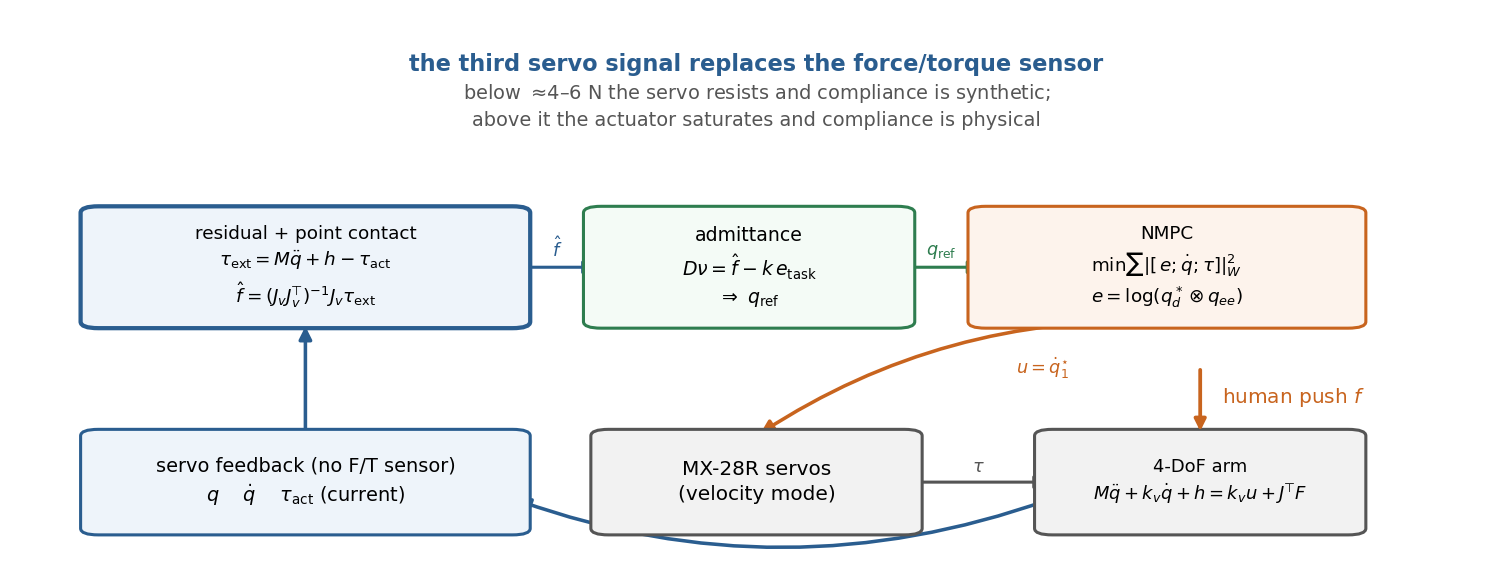
\includegraphics[width=0.95\textwidth]{architecture.png}
\caption{System architecture. The servo returns position, velocity, and effort;
the effort channel takes the place of a force/torque sensor. The residual and the
point-contact inversion produce $\hat{\bm f}$, an admittance converts it into a
displaced pose reference, and the predictive controller returns a joint
velocity command, which is the only input the actuator accepts.}
\label{fig:arch}
\end{figure*}

\subsection{The velocity-actuated plant}
\label{sec:velplant}
Since the actuator is commanded in velocity, the plant seen by the controller is
not \eqref{eq:dyn}. Modeling the internal servo loop as a proportional velocity
regulator,
\begin{equation}
\bm\tau=k_v\,(\bm u-\dot{\bm q}),
\label{eq:servoloop}
\end{equation}
and substituting into \eqref{eq:dyn} gives the closed-loop plant in compact form,
\begin{equation}
\boxed{\;\bm M(\bm q)\,\ddot{\bm q}+k_v\,\dot{\bm q}+\bm h(\bm q,\dot{\bm q})
=k_v\,\bm u+\Jfull(\bm q)^{\!\top}\bm F\;}
\label{eq:velplant}
\end{equation}
which we verified against \eqref{eq:dyn} to $4.3\times10^{-14}$ over randomized
states, gains, and wrenches. Equation \eqref{eq:velplant} makes the role of the
servo explicit: it contributes a damping term $k_v\bm I$ and an input gain $k_v$,
and as $k_v\to\infty$ it degenerates to the kinematic limit $\dot{\bm q}=\bm u$ in
which the arm is a pure velocity source. Actuator saturation enters as
$\norm{\bm\tau}_\infty\le\tau_{\max}$ applied to \eqref{eq:servoloop}, and
Section~\ref{sec:velocity-regimes} shows that this bound, rather than the loop
gain, is what governs the interaction.

\begin{remark}[The estimator does not use $k_v$]
Equation \eqref{eq:servoloop} is written for analysis only. The residual
\eqref{eq:residual} uses $\tauact$ as \emph{measured} through the effort channel,
not as modeled, so $k_v$ appears nowhere in the estimator. We verified that the
recovered force is identical for $k_v\in\{1,10,100\}$. The internal servo loop may
therefore remain a black box, and no system identification of it is required. This
is the formal reason why velocity-level actuation does not obstruct sensorless
estimation.
\label{rem:kv}
\end{remark}

\subsection{Pose error}
\label{sec:poseerr}
Tracking requires a scalar measure of pose error. We use a six-dimensional error
whose rotational part is the axis-angle vector $\bm\varphi$ of the orientation
error and whose translational part is expressed in the frame of that rotational
error,
\begin{equation}
\bm e=\begin{bmatrix}\bm\varphi\\ \bm\rho\end{bmatrix}\in\R^{6},
\qquad
\bm\rho=\bm J_\ell(\bm\varphi)^{-1}\bm t_{\mathrm{err}},
\label{eq:logdual}
\end{equation}
with $\bm J_\ell$ the left Jacobian of $\mathrm{SO}(3)$~\cite{sola2018microlie}
and $\bm t_{\mathrm{err}}$ the translational error. The factor
$\bm J_\ell^{-1}$ is what distinguishes \eqref{eq:logdual} from a decoupled
error that adds position and orientation independently, and since
$\bm J_\ell^{-1}\to\bm I$ as $\|\bm\varphi\|\to0$ the two agree in the
small-error limit. The choice matters only for the demonstrator and carries no
weight in the contributions of this paper; we adopt \eqref{eq:logdual} because it
supplies a geometrically consistent compromise by construction and at no
computational cost, both variants requiring $2.48$~ms per solve.

\subsection{Model validation}
\label{sec:validation}
The symbolic model was built independently of the simulator and validated against
MuJoCo~\cite{todorov2012mujoco} over eight configurations spanning the joint
ranges (Table~\ref{tab:validation}). The agreement is at the numerical precision
of the reference implementation, so modeling error is not a confounding factor in
what follows. This matters, because the central claim of this paper is that an
observed estimation error belongs to the inversion step, and that attribution is
credible only if the model itself is exact.

\begin{table}[!t]
\caption{Model validation against MuJoCo, eight configurations.}
\label{tab:validation}
\centering
\small
\begin{tabular}{lc}
\toprule
quantity & maximum deviation\\
\midrule
inertia matrix $\bm M$          & $8.8\times10^{-11}$\\
bias term $\bm h$               & $2.7\times10^{-9}$\\
forward kinematics, position    & $6.9\times10^{-13}$~m\\
forward kinematics, orientation & $0$ (machine precision)\\
geometric Jacobian $\Jfull$     & $4\times10^{-17}$\\
\bottomrule
\end{tabular}
\end{table}

% =========================================================================
\section{Contact-Model-Aware Force Estimation}
\label{sec:estimation}
% =========================================================================

\subsection{The residual and the estimation problem}
Rearranging \eqref{eq:dyn} gives the measurable residual
\begin{equation}
\tauext=\bm M(\bm q)\ddot{\bm q}+\bm h(\bm q,\dot{\bm q})-\tauact
=\Jfull(\bm q)^{\!\top}\bm F \;\in\;\R^{4},
\label{eq:residual}
\end{equation}
computed from joint measurements alone: $\bm q$ and $\dot{\bm q}$ from encoders,
$\ddot{\bm q}$ by finite differences, and $\tauact$ from the servo current.
Everything the arm knows about the interaction is in these four numbers.

\begin{problem}
Given $\tauext\in\R^4$ from \eqref{eq:residual}, recover the external contact
force acting at the end-effector, and characterize the configurations in which
recovery is possible and the accuracy attainable.
\label{prob:main}
\end{problem}

Problem~\ref{prob:main} asks for a \emph{force}, not a wrench. That distinction is
the substance of this section: the number of unknowns admitted into the inversion
determines whether the problem is solvable, and the conventional choice admits too
many.

\subsection{The six-dimensional inversion}
The conventional estimator treats the full wrench as unknown and solves
$\Jfull^{\!\top}\bm F=\tauext$ for $\bm F\in\R^6$ from four equations. The system
is under-determined and the minimum-norm solution is
\begin{equation}
\hat{\bm F}_{6}=\Jfull\big(\Jfull^{\!\top}\Jfull\big)^{-1}\tauext=\Pobs\,\bm F,
\quad
\Pobs=\Jfull\big(\Jfull^{\!\top}\Jfull\big)^{-1}\Jfull^{\!\top},
\label{eq:sixinv}
\end{equation}
with $\Pobs$ the orthogonal projector onto $\mathrm{col}\,\Jfull\subset\R^6$.

\begin{proposition}[Force-to-moment misattribution]
For a pure contact force $\bm F=[\bm f^{\!\top}\ \bm 0^{\!\top}]^{\!\top}$, the
force returned by \eqref{eq:sixinv} is $\Pff\bm f$, where $\Pff$ is the leading
$3\times3$ block of $\Pobs$. In general $\norm{\Pff\bm f}<\norm{\bm f}$, and the
deficit appears as a nonzero moment in the lower block of $\hat{\bm F}_{6}$.
\label{prop:split}
\end{proposition}

The mechanism is misattribution, not loss of information. A pure force and a
suitable force-moment pair produce identical joint torques, and minimum-norm
selects the latter because it has smaller Euclidean norm in $\R^6$. Both are
consistent with the measurement; only one is realizable by the contact under
consideration, and nothing in the formulation encodes which.

At the task configuration $\bm q_{\text{task}}=[0,\,1.2,\,-0.9,\,0.4]$~rad, a
$6$~N push normal to the plane of the arm produces
$\tauext=[1.2867,\,0,\,0,\,0]^{\!\top}\,\mathrm{N}\cdot\mathrm{m}$. Equation
\eqref{eq:sixinv} returns $0.264$~N of force together with
$1.230\,\mathrm{N}\cdot\mathrm{m}$ of moment. The eigenvalues of $\Pff$ there are
$\{0.044,\,1,\,1\}$: two force directions pass unaltered while a third is almost
entirely converted into a moment.

\begin{remark}[Aggregate observability is uninformative]
Since $\Pobs$ is an orthogonal projector, $\mathrm{tr}\,\Pobs=\mathrm{rank}\,
\Jfull$ identically, so for wrench directions drawn uniformly on the unit sphere
of $\R^6$ the expected fraction returned by \eqref{eq:sixinv} is
$\mathrm{rank}\,\Jfull/6$ regardless of configuration. Any workspace-averaged
observability index built on $\Pobs$ is constant by construction and carries no
information about posture. The structure lies in how the deficit is distributed
across directions.
\label{rem:trace}
\end{remark}

\begin{remark}[Numerical care at singularities]
At singular configurations $\Jfull$ loses rank and \eqref{eq:sixinv} is undefined.
Throughout this work $\Pobs$ is computed from the thin singular value
decomposition $\Jfull=\bm U\bm\Sigma\bm V^{\!\top}$ as
$\Pobs=\bm U_r\bm U_r^{\!\top}$ with $r$ the numerical rank, which remains valid
there.
\end{remark}

\subsection{The point-contact inversion}
A human push at the end-effector transmits a force at a known point and no moment
about that point. Imposing $\bm m=\bm 0$ in \eqref{eq:residual} leaves
\begin{equation}
\Jv(\bm q)^{\!\top}\,\bm f=\tauext,\qquad \Jv^{\!\top}\in\R^{4\times3},
\label{eq:threeinv}
\end{equation}
over-determined: four equations in three unknowns, with least-squares solution
\begin{equation}
\hat{\bm f}_{3}=\big(\Jv\Jv^{\!\top}\big)^{-1}\Jv\,\tauext .
\label{eq:threesol}
\end{equation}

\begin{proposition}[Exact recovery]
$\hat{\bm f}_{3}=\bm f$ for every pure contact force applied at the end-effector
if and only if $\mathrm{rank}\,\Jv=3$. The result is independent of the rank
deficit of $\Jfull$ and does not involve $\Jw$.
\label{prop:exact}
\end{proposition}

\begin{proof}
By construction \eqref{eq:threeinv} is consistent, since $\tauext=\Jv^{\!\top}
\bm f$ for the true $\bm f$. A consistent least-squares problem attains zero
residual, and its solution is unique precisely when $\Jv^{\!\top}$ has trivial
kernel, that is when $\mathrm{rank}\,\Jv=3$. If $\mathrm{rank}\,\Jv<3$ the
solution set is an affine subspace of dimension $3-\mathrm{rank}\,\Jv$ and
\eqref{eq:threesol} returns its minimum-norm element, which differs from $\bm f$
whenever $\bm f$ has a component in $\ker\Jv^{\!\top}$. The angular block $\Jw$
appears nowhere in \eqref{eq:threeinv}, so the rank of $\Jfull$ is irrelevant.
\end{proof}

Proposition~\ref{prop:exact} moves the governing condition from
$\Jfull\in\R^{6\times4}$, which cannot attain rank $6$, to $\Jv\in\R^{3\times4}$,
which generically attains rank $3$. Four joints are not too few to sense a contact
force at the end-effector; they are one more than the minimum required.

\begin{remark}[What the model assumption costs]
The point-contact model requires the contact location to be known. This holds for
hand guiding at the end-effector and fails for contact along the links. If the
contact additionally transmits a moment, for instance through a rigidly grasped
object, the ambiguity of Proposition~\ref{prop:split} returns and
\eqref{eq:sixinv} becomes the honest choice, with the accompanying loss. Relaxing
the assumption is an established line in its own right: the contact location can be
recovered together with the force by constrained
optimization~\cite{likar2014contact} or by particle filtering over the
robot surface~\cite{manuelli2016cpf}, and it is what the virtual force sensor
provides on redundant arms~\cite{magrini2014virtual}. Extending the estimator in
that direction is future work.
\label{rem:cost}
\end{remark}

\subsection{Conditioning as the binding limitation}
\label{sec:conditioning}
With exactness settled, the practically relevant quantity is sensitivity to
measurement noise. Perturbing the residual by $\delta\bm\tau$ perturbs the
estimate by
\begin{equation}
\norm{\delta\hat{\bm f}_{3}}\le\frac{\norm{\delta\bm\tau}}{\sigma_{\min}(\Jv)} ,
\label{eq:noise}
\end{equation}
so $\sigma_{\min}(\Jv)$ bounds the amplification of residual error into force
error and replaces observability as the quantity to map.

That Jacobian conditioning governs the accuracy of residual-based force estimation
is established. Lu \emph{et al.} bound the relative force error of a six-joint
industrial robot by the condition number of $\bm J^{\!\top}$ times the relative
residual error, map that condition number over half a million sampled
configurations, and then optimize the task path and end-effector pose to lower it,
thereby suppressing the effect of modeling error without reducing the error
itself~\cite{lu2023configopt}.

Three things differ here, and they follow from the regime rather than from the
technique. Their reconstruction inverts $\bm J^{\!\top}$ directly, which presumes
it is square and invertible; for $n<6$ that inverse does not exist, and
\eqref{eq:noise} is instead an absolute bound on the over-determined point-contact
inverse \eqref{eq:threesol}, whose relevant quantity is the smallest singular value
of $\Jv$ rather than a condition number of $\Jfull$. Their workspace study maps the
\emph{index}; Section~\ref{sec:sweep} maps the \emph{error}, and shows that its
dominant component is the structural misattribution of
Proposition~\ref{prop:split}, which survives at good conditioning and therefore
cannot be removed by any posture choice. And where a six-joint arm executing a
one-dimensional path has a redundant angle to spend on conditioning, a four-joint
arm tracking a pose has none, so $\sigma_{\min}(\Jv)$ is used here as a gate that
declines to report rather than as an objective to maximize. The bound is verified
as a law on the simulated plant in Section~\ref{sec:res-cond}.

\subsection{Workspace characterization}
\label{sec:sweep}
We sweep the three pitch joints over their full ranges on a $13^3$ grid, fixing
the base yaw since it only rotates the picture in the world frame and leaves every
quantity of interest invariant. This gives $2197$ configurations, at each of which
we compute the rank and singular values of $\Jv$ and apply a random unit contact
force, recording the error of both estimators. Table~\ref{tab:sweep} summarizes
and Fig.~\ref{fig:map} maps the outcome.

\begin{table*}[!t]
\caption{Workspace sweep over $2197$ configurations. The contact force is exactly
recoverable everywhere by the point-contact estimator, while the six-dimensional
inversion discards half of it on average.}
\label{tab:sweep}
\centering
\small
\begin{tabular}{lcccc}
\toprule
quantity & mean & median & 5th percentile & extreme\\
\midrule
$\sigma_{\min}(\Jv)$ & $0.0500$ & $0.0496$ & $0.0127$ & $7.6\times10^{-5}$ (min)\\
$\mathrm{cond}(\Jv)$ & --- & $6.7$ & --- & $29.4$ (95th percentile)\\
$\mathrm{rank}\,\Jv=3$ & \multicolumn{4}{c}{$100\,\%$ of configurations}\\
\midrule
\multicolumn{5}{l}{\emph{error estimating a unit contact force}}\\
six-dimensional, $\norm{\hat{\bm f}_{6}-\bm f}$ & $0.5046$ & $0.5110$ & --- & $0.9961$ (max)\\
point contact, $\norm{\hat{\bm f}_{3}-\bm f}$ & $3.6\times10^{-15}$ & $7.1\times10^{-16}$ & --- & $1.4\times10^{-12}$ (max)\\
\bottomrule
\end{tabular}
\end{table*}

Two facts stand out. First, $\mathrm{rank}\,\Jv=3$ in $100\,\%$ of the grid, so by
Proposition~\ref{prop:exact} the contact force is exactly recoverable everywhere,
and the numerical error of $\hat{\bm f}_{3}$ is at machine precision. Second, over
the same set the six-dimensional inversion discards $50.5\,\%$ of the applied
force on average and, in the worst configuration and direction, essentially all of
it.

\begin{figure*}[!t]
\centering
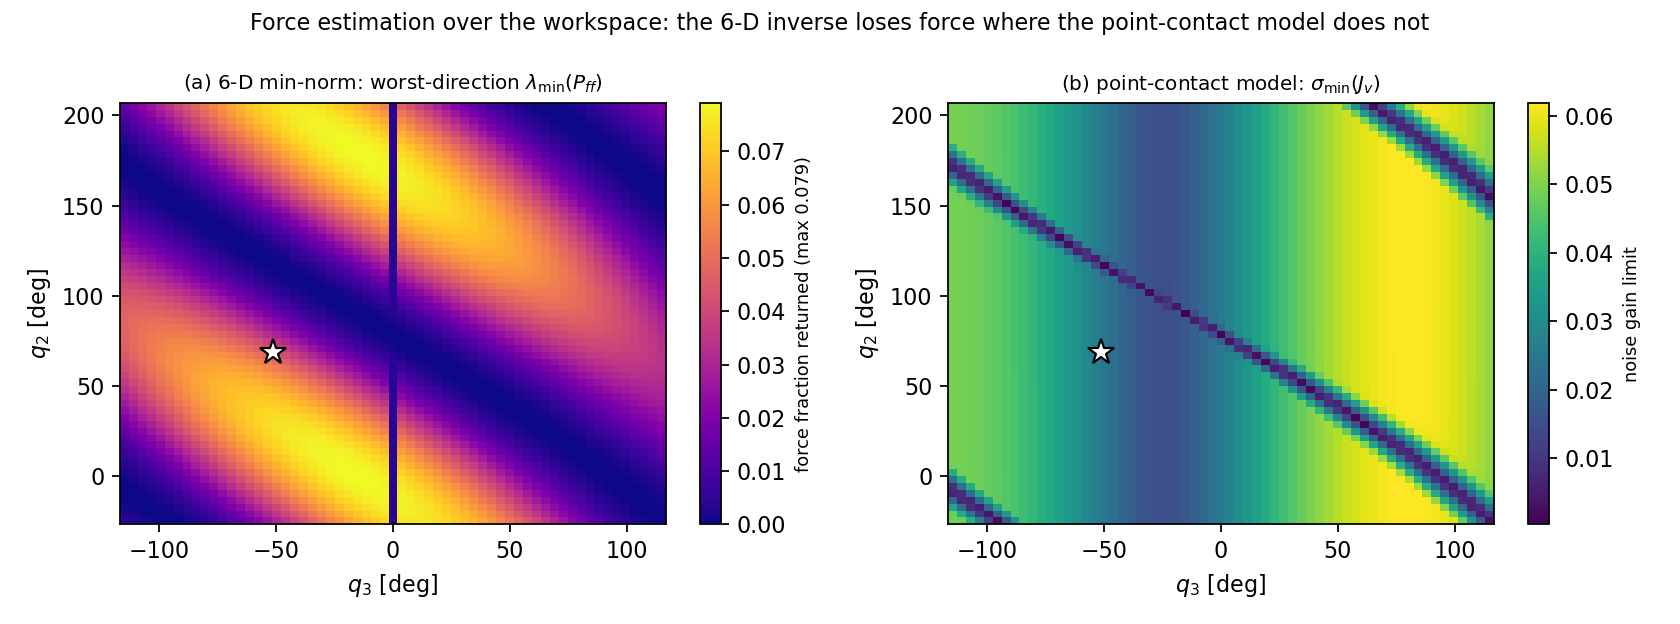
\includegraphics[width=0.92\textwidth]{observability_map.png}
\caption{Force estimation over a slice of the workspace ($q_1=0$, $q_4=0.4$~rad).
(a) Worst-direction eigenvalue of $\Pff$, the fraction of a pure contact force
that the six-dimensional inversion returns as force; close to zero throughout,
which is the effect that has been misread as blindness of the mechanism.
(b) $\sigma_{\min}(\Jv)$, which bounds noise amplification for the point-contact
inversion and is the quantity that actually limits it. The star marks the task
configuration.}
\label{fig:map}
\end{figure*}

The geometric reason the six-dimensional inversion fails in a particular direction
is worth stating, because it explains why the effect is systematic on this class
of arm. The three pitch joints are coplanar, so the torques they produce resist
only loads in the plane of the arm. A force component normal to that plane reaches
the actuators through a single path, the moment it exerts about the base yaw axis.
A moment applied directly about that same axis produces the identical joint torque
with a smaller norm in $\R^6$, so the minimum-norm criterion prefers it. The
out-of-plane force direction is therefore exactly the one that the
six-dimensional inversion converts into a moment, in every configuration of this
architecture.

\subsection{Directional characterization}
\label{sec:dirsweep}
The preceding argument predicts that the error of the six-dimensional inversion is
governed by the \emph{direction} of the push and by nothing else. That prediction
is falsifiable and we test it directly, since a claim of this kind cannot rest on
the two push directions used in the closed-loop experiments of
Section~\ref{sec:res-estimation}. We sweep the full sphere of push directions,
$2000$ uniformly drawn directions at each of six configurations spread over the
workspace, and for each direction record the relative error of both inversions
together with the alignment $|\cos\theta|$ between the push and the least
observable eigenvector of $\Pff$ at that pose.

\begin{table}[!t]
\caption{Directional sweep. Relative force error over $2000$ push directions at
each of six configurations.}
\label{tab:dirsweep}
\centering
\footnotesize
\setlength{\tabcolsep}{4pt}
\begin{tabular}{lccccc}
\toprule
& & \multicolumn{3}{c}{six-dimensional [\%]} & point contact\\
\cmidrule(lr){3-5}
pose & $\sigma_{\min}(\Jv)$ & median & p90 & max & max [\%]\\
\midrule
P1 & $0.0255$ & $47.7$ & $85.7$ & $95.6$ & $4.1\times10^{-13}$\\
P2 & $0.0357$ & $49.5$ & $89.7$ & $99.6$ & $1.9\times10^{-13}$\\
P3 & $0.0597$ & $49.1$ & $86.3$ & $96.5$ & $1.9\times10^{-13}$\\
P4 & $0.0403$ & $48.1$ & $89.6$ & $99.8$ & $2.2\times10^{-13}$\\
P5 & $0.0802$ & $48.8$ & $85.5$ & $94.9$ & $1.5\times10^{-13}$\\
P6 & $0.0303$ & $48.0$ & $87.7$ & $97.3$ & $2.0\times10^{-13}$\\
\bottomrule
\end{tabular}
\end{table}

Table~\ref{tab:dirsweep} reports the result. Three observations follow. The median
error of the six-dimensional inversion is between $47.7$ and $49.5\,\%$ at every
pose, and roughly half of all push directions incur an error above $50\,\%$, so
the failure is not confined to a special direction or a special posture. The
point-contact inversion is exact to $4\times10^{-13}\,\%$ over all $12\,000$
directions and all six poses. And the poses span $\sigma_{\min}(\Jv)$ from
$0.0255$ to $0.0802$ without the six-dimensional error responding, confirming that
its error is not a conditioning effect.

\begin{figure*}[!t]
\centering
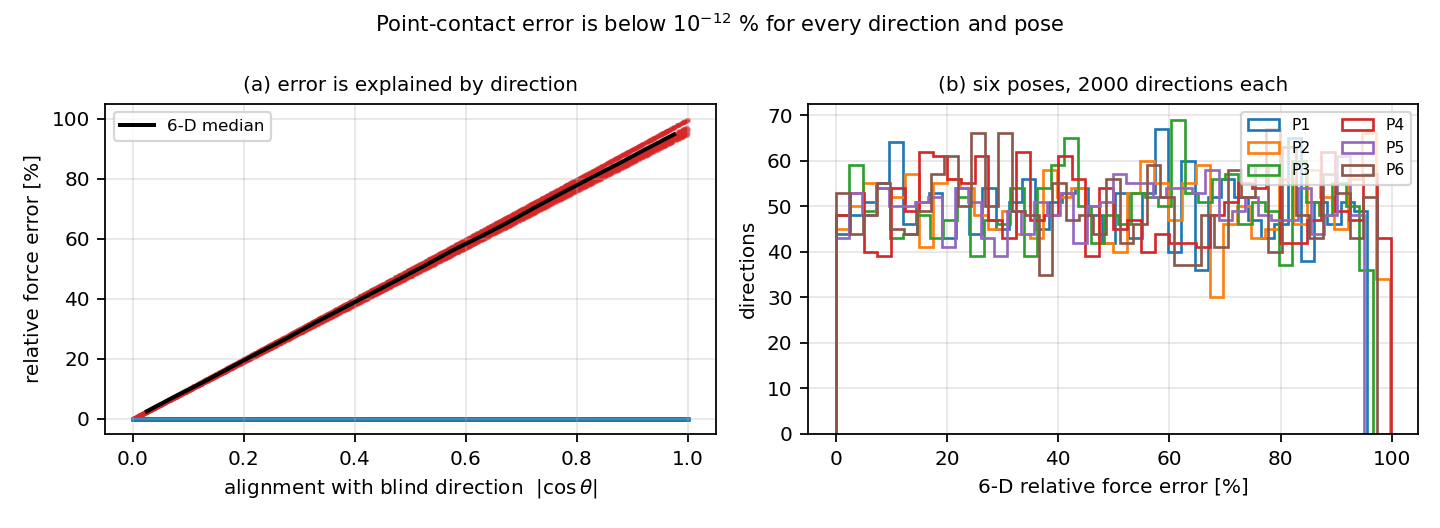
\includegraphics[width=0.92\textwidth]{direction_sweep.png}
\caption{Directional sweep over $12\,000$ push directions at six configurations.
(a) Relative force error against alignment with the least observable direction:
the six-dimensional error (red) is a linear function of alignment with correlation
$0.9993$, while the point-contact error (blue) lies at zero. (b) Error
distributions of the six-dimensional inversion at each pose, which coincide,
showing the effect is a property of the architecture rather than of a posture.}
\label{fig:dirsweep}
\end{figure*}

Fig.~\ref{fig:dirsweep} confirms the mechanism quantitatively. Pooling the
$12\,000$ directions, the median six-dimensional error grows monotonically with
alignment, from $9.8\,\%$ below $|\cos\theta|=0.2$ to $94.8\,\%$ above $0.95$, and
the correlation between alignment and error is $0.9993$. The geometric explanation
is therefore not an interpretation placed on the numbers after the fact: it
accounts for essentially all of the variance.

\begin{remark}[Scope of the correlation]
The least observable direction is obtained from $\Pff$, that is from the same
model that produces the error, so the correlation of $0.9993$ should be read for
what it is: evidence that a single scalar function of the push direction predicts
the error, not an independent confirmation. What it excludes is that the error
depends on magnitude, on posture, or on conditioning, all of which are varied
across the sweep without affecting it. An independent test would identify the
least observable direction empirically on hardware and check that it coincides
with the one $\Pff$ predicts.
\end{remark}

% =========================================================================
\section{Estimation Under Velocity-Level Actuation}
\label{sec:velocity}
% =========================================================================

The residual \eqref{eq:residual} is written in torque, while the actuator accepts
velocity. This section shows that the mismatch is apparent, that velocity-level
actuation in fact simplifies the estimation problem, and that it changes both the
error budget and the nature of the compliance obtained.

Remark~\ref{rem:kv} already established the structural point: the residual uses
$\tauact$ as measured through the effort channel, so the servo gain $k_v$ does not
enter the estimator and the inner loop need not be identified. What must be known
is the map from reported current to torque, which is a calibration rather than a
system identification. The remainder of this section works out the quantitative
consequences.

\subsection{Where the interaction signal appears}
\label{sec:velocity-signal}
Simulating the plant \eqref{eq:velplant} under a $6$~N push at
$\bm q_{\text{task}}$, and holding $\bm u=\bm 0$ so that the servo attempts to
keep the arm still, the residual \eqref{eq:residual} splits between its inertial
term $\bm M\ddot{\bm q}$ and its actuator term $\bm h-\tauact$ as reported in
Table~\ref{tab:velocity}.

\begin{table}[!t]
\caption{Distribution of the residual as a function of velocity-loop stiffness,
for a $6$~N push.}
\label{tab:velocity}
\centering
\footnotesize
\setlength{\tabcolsep}{4pt}
\begin{tabular}{ccccc}
\toprule
$k_v$ & $\norm{\bm M\ddot{\bm q}}$ & $\norm{\bm h-\tauact}$
& in $\tauact$ & displacement\\
\midrule
$1$   & $0.0147$   & $0.596$ & $97.6\,\%$  & $350$~mm\\
$4$   & $0.0008$   & $1.426$ & $99.9\,\%$  & $106$~mm\\
$20$  & $0.0001$   & $1.314$ & $100.0\,\%$ & $18$~mm\\
$100$ & $\approx0$ & $1.291$ & $100.0\,\%$ & $3.5$~mm\\
\bottomrule
\end{tabular}
\end{table}

For any realistic loop gain the force appears almost entirely in $\tauact$. The
servo rejects the disturbance, the arm barely moves, and the interaction is
expressed as the torque the actuator must produce in order not to move. Two
consequences follow, and they redirect the engineering effort in a way that is not
obvious beforehand.

First, the finite-differenced acceleration, normally the delicate quantity in a
residual observer, becomes irrelevant: it carries $0.006\,\%$ of the signal.
Effort spent filtering encoder differences is misplaced on this platform.

Second, the entire error budget transfers to the current-to-torque calibration,
where sensitivity is one to one: a $5\,\%$ error in the torque constant produces a
$5\,\%$ error in force. A torque offset is milder, $0.05\,\mathrm{N}\cdot\mathrm{m}$
per joint producing $3.7\,\%$.

\subsection{Detection floor}
Combining Section~\ref{sec:velocity-signal} with \eqref{eq:noise} gives the
smallest force distinguishable from residual error. A residual error of
$0.01\,\mathrm{N}\cdot\mathrm{m}$ corresponds to $0.20$~N at the median posture,
$0.79$~N at the fifth percentile of $\sigma_{\min}(\Jv)$, and is unusable at the
worst posture. Since the dominant term on a small geared servo is stiction, of
order $0.05\,\mathrm{N}\cdot\mathrm{m}$, the expected floor is one to two newtons
at a typical posture. This is adequate for hand guiding with pushes of five to
fifteen newtons, and it is the quantity that governs the design.

\subsection{Two compliance regimes}
\label{sec:velocity-regimes}
Because the servo behaves as a velocity source, the arm does not yield under a
push of its own accord, and compliance must be produced by displacing the
reference: sense, move the reference, track. This synthetic compliance is limited
by loop latency rather than by any physical property.

That description is only half correct, and the missing half is favorable. The
actuator torque is bounded, so the force the arm can exert is bounded as well.
Sweeping $729$ configurations and evaluating the worst direction at each,
subject to $|\tau_i|\le1.4\,\mathrm{N}\cdot\mathrm{m}$ and supporting the arm's own
weight, the maximum exertable force has median $5.88$~N, fifth percentile
$4.29$~N, and minimum $3.93$~N. Manual guidance requires five to fifteen newtons.
The interaction therefore has two regimes:

\begin{itemize}[leftmargin=*]
\item \emph{Below roughly $4$ to $6$~N.} The servo resists, the arm barely moves,
and compliance is synthetic. Loop latency governs how the interaction feels.
\item \emph{Above that threshold.} The actuator saturates and the arm is displaced
until it reaches a posture where it can hold the load. Compliance is physical and
obtained for free.
\end{itemize}

The transition between the two is not a matter of interpretation. It has a
measurable signature: below the threshold the arm follows the reference the
admittance commands, while above it the actuator saturates and the arm is carried
further than commanded. Table~\ref{tab:regimes} reports the ratio of actual to
commanded end-effector displacement in the closed compliant loop under pushes of
increasing magnitude.

\begin{table}[!t]
\caption{The two compliance regimes. Steady-state end-effector displacement,
actual versus commanded by the admittance, under a push of increasing magnitude.}
\label{tab:regimes}
\centering
\footnotesize
\setlength{\tabcolsep}{5pt}
\begin{tabular}{ccccc}
\toprule
$\norm{\bm f}$ [N] & commanded [mm] & actual [mm] & ratio & saturated steps\\
\midrule
$1$  & $8.3$   & $8.6$   & $1.03$ & $0\,\%$\\
$3$  & $24.8$  & $23.7$  & $0.95$ & $0\,\%$\\
$5$  & $41.4$  & $37.8$  & $0.91$ & $0\,\%$\\
\midrule
$6$  & $49.7$  & $86.0$  & $1.73$ & $100\,\%$\\
$8$  & $66.2$  & $124.5$ & $1.88$ & $98\,\%$\\
$10$ & $82.8$  & $162.3$ & $1.96$ & $98\,\%$\\
$15$ & $124.1$ & $207.8$ & $1.67$ & $99\,\%$\\
\bottomrule
\end{tabular}
\end{table}

The transition falls between $5$ and $6$~N, in agreement with the actuator capability
computed independently above, and the two indicators change together: the ratio
departs from unity exactly where the saturated fraction goes from none to all.

The arm is thus naturally backdrivable in the regime of interest, which is a
safety property rather than a deficiency, and the synthetic loop only has to cover
fine guidance and the return to task. Two practical consequences follow. The
latency requirement on the control loop is milder than a purely synthetic analysis
would suggest, since above the threshold the physics yields without waiting for
the loop. And actuator sizing becomes a compliance design variable: choosing a
servo whose force capability falls below the expected interaction range confers
intrinsic backdrivability with no control effort at all.

\begin{remark}[The estimator does not saturate]
One might expect the estimate to saturate together with the actuator. It does not.
Under a force ramp with $|\tau_i|\le1.4\,\mathrm{N}\cdot\mathrm{m}$ the estimate
remains exact across the range, returning $1.000$, $5.999$, and $13.998$~N for
applied magnitudes of $1$, $6$, and $14$~N, an error of $0.0\,\%$ throughout. The
reason is that the residual \eqref{eq:residual} contains both terms: when the
actuator can no longer hold, the arm accelerates and redistributes its posture,
and the balance shifts from $\tauact$ towards $\bm M\ddot{\bm q}$ and towards a
configuration in which the load can be supported. The formulation captures both
regimes without modification.
\end{remark}

% =========================================================================
\section{Compliant Control: An Integration Demonstrator}
\label{sec:control}
% =========================================================================

\subsection{Admittance}
The estimated contact force drives a first-order admittance that displaces the
reference pose from the nominal task pose, with a return spring that restores it
when contact ceases,
\begin{equation}
\bm D\,\bm\nu = \hat{\bm f}_{3} - k\,\bm e_{\mathrm{task}},
\label{eq:admittance}
\end{equation}
where $\bm\nu$ is the reference twist, $\bm D$ collects translational and
rotational damping, $k$ is the return stiffness, and $\bm e_{\mathrm{task}}$ is the
displacement of the reference from the task pose. The twist is integrated on the
dual pose reference directly, so translation and rotation remain one object.

\subsection{Predictive controller}
A nonlinear predictive controller tracks the compliant reference. The state is
$\bm x=[\bm q^{\!\top}\ \dot{\bm q}^{\!\top}]^{\!\top}\in\R^8$, the input is joint
torque, and the servo receives the predicted velocity $\dot{\bm q}^\star_1$, which
matches its native command mode. The optimal control problem is
\begin{equation}
\begin{aligned}
\min_{\bm x,\bm\tau}\quad
&\sum_{k=0}^{N-1}\norm{\bm y_k}^2_{\bm W}+\norm{\bm y_N}^2_{\bm W_N}\\
\mathrm{s.t.}\quad
&\bm x_0=\hat{\bm x},\qquad \bm x_{k+1}=\bm\Phi(\bm x_k,\bm\tau_k),\\
&\bm q_{\min}\le\bm q_k\le\bm q_{\max},\quad
\norm{\dot{\bm q}_k}_\infty\le\dot q_{\max},\\
&\norm{\bm\tau_k}_\infty\le\tau_{\max},
\end{aligned}
\label{eq:ocp}
\end{equation}
with residual $\bm y=[\bm e^{\!\top}\ \dot{\bm q}^{\!\top}\ \bm\tau^{\!\top}]^{\!\top}$
built on \eqref{eq:logdual}, and $\bm\Phi$ the discretized dynamics \eqref{eq:dyn}
with $\bm F=\bm 0$, since the interaction enters through the reference rather than
the prediction model. The horizon is $N=20$ nodes over $1.0$~s.

\subsection{Which model should the controller use?}
\label{sec:whichmodel}
Formulation \eqref{eq:ocp} takes torque as the decision variable while the
actuator accepts velocity, so the predicted velocity is passed to the servo. This
is the customary arrangement, but on velocity-actuated hardware it is not the only
one, and the alternatives differ in what they require the designer to know. We
implemented and compared three.

\begin{itemize}[leftmargin=*]
\item \textbf{T}, torque level: $\bm x=[\bm q,\dot{\bm q}]$, $\bm u=\bm\tau$, the
dynamics \eqref{eq:dyn}, with $\dot{\bm q}^\star_1$ sent to the servo. Requires
$\bm M$ and $\bm h$. Does not require $k_v$.
\item \textbf{V1}, dynamic velocity level: $\bm x=[\bm q,\dot{\bm q}]$, $\bm u$ the
velocity command, the plant \eqref{eq:velplant}. Requires $\bm M$, $\bm h$
\emph{and} $k_v$, that is, identification of the servo loop.
\item \textbf{V0}, kinematic: $\bm x=[\bm q]$, $\bm u$ the velocity command,
$\dot{\bm q}=\bm u$, the limit of \eqref{eq:velplant} as $k_v\to\infty$. Requires
nothing: no inertia, no bias term, no servo gain.
\end{itemize}

\begin{table}[!t]
\caption{Controller formulations under velocity-level actuation. Regulation to a
fixed pose from an initial error of $0.16$~m, on the plant \eqref{eq:velplant}
with torque saturation.}
\label{tab:formulations}
\centering
\footnotesize
\setlength{\tabcolsep}{3.5pt}
\begin{tabular}{lccccc}
\toprule
 & $n_x$ & needs $\bm M,\bm h$ & needs $k_v$ & error [mm] & ms/solve\\
\midrule
T  & $8$ & yes & no  & $0.180$ & $2.60$\\
V1 & $8$ & yes & \textbf{yes} & \emph{fails} & $2.67$\\
V0 & $4$ & no  & no  & $\bm{0.120}$ & $\bm{0.10}$\\
\bottomrule
\end{tabular}
\vspace{2pt}
\\{\footnotesize Error after settling; V0 with command weight tuned. V1 returns
\texttt{NAN\_DETECTED} at every solve, see text.}
\end{table}

Table~\ref{tab:formulations} reports the comparison, and the outcome is not the
expected one.

\emph{V1 is ill-posed.} Every solve fails. The cause is instructive rather than
numerical: with a proportional loop model, sustaining a velocity requires a
persistent velocity error, so imposing the true actuator bound
$|k_v(u_i-\dot q_i)|\le\tau_{\max}$ restricts the command to
$|u_i|\le\tau_{\max}/k_v=0.07$~rad/s, which is $85$ times below the
$5.969$~rad/s the servo actually reaches. Omitting the bound is worse, since the
model then admits torques of $239\,\mathrm{N}\cdot\mathrm{m}$, two orders of
magnitude beyond the actuator, and the integrator diverges. The defect is the
model structure: the real servo loop has integral action, so no persistent torque
is needed to hold a velocity. Formulating V1 correctly therefore requires
identifying not only a gain but the loop architecture including anti-windup, which
is precisely the burden the other two formulations avoid.

\emph{V0 needs no model at all and is not worse.} Once the command weight is
tuned it settles to $0.120$~mm against $0.180$~mm for T, at $0.086$~ms per solve,
a factor of thirty faster, with no failures. Its state is half the size and it
uses neither the inertia matrix nor the bias term.

This yields a clean separation of concerns, which we regard as the practical
recommendation of this paper:

\begin{quote}
\emph{On a velocity-actuated arm the dynamic model is required by the
\textbf{estimator} and by nothing else. The controller can be model-free.}
\end{quote}

The estimator needs $\bm M$ and $\bm h$ to form the residual \eqref{eq:residual},
and by Remark~\ref{rem:kv} it needs no knowledge of the servo loop. The controller
needs neither. The only quantities to be identified on hardware are therefore the
kinematics, the mass properties, and the current-to-torque constant, all of which
serve estimation, and none of which serve control.

\begin{remark}[What V0 gives up]
The kinematic formulation cannot express torque bounds, so it cannot by itself
prevent commands the actuator will not follow. Two considerations make this
acceptable here. The velocity bound is retained and is the binding limit in normal
operation, and by Section~\ref{sec:velocity-regimes} exceeding the torque bound
does not produce a fault but the physically compliant regime, in which the arm
yields. If a hard torque bound is required, for instance to protect a payload, the
static requirement $\norm{\bm h(\bm q)+\Jv^{\!\top}\hat{\bm f}}_\infty\le\tau_{\max}$
can be imposed on V0 as a state constraint without reintroducing $k_v$.
\end{remark}

Table~\ref{tab:formulations} compares the three under regulation. The claim that
the controller can be model-free is stronger than a regulation test, however, so
Section~\ref{sec:res-model} repeats the complete compliant interaction loop with
V0 in place of T.

Problem \eqref{eq:ocp} is transcribed with CasADi~\cite{andersson2019casadi} and
solved by the real-time iteration scheme~\cite{diehl2005rti} in
acados~\cite{verschueren2022acados}, with HPIPM~\cite{frison2020hpipm}, a
Gauss-Newton Hessian, and a fourth-order explicit Runge-Kutta integrator.

Because $n=4$, a general $\SEthree$ reference is unreachable and the optimizer
settles on a compromise between orientation and translation error. Which
compromise it selects is decided by the metric, which is what
$\bm J_\ell^{-1}$ in \eqref{eq:logdual} supplies.

\subsection{Real-time implementation}
\label{sec:realtime}
Reaching real-time rates required one change whose effect is disproportionate to
its visibility, and which we report because the failure mode is easy to reach and
hard to diagnose.

In an initial implementation the symbolic model was assembled with the
graph-valued expression type of CasADi and the forward dynamics written as
$\ddot{\bm q}=\mathrm{solve}(\bm M,\bm\tau-\bm h)$. On graph-valued operands this
does not produce a closed-form expression: it emits a node backed by a numerical
QR factorization, whose derivatives are obtained by implicit differentiation of
the linear system and which cannot be expanded to scalar form. With a four-stage
explicit integrator propagating sensitivities across twenty nodes, that routine is
evaluated approximately eighty times per solve. The measured cost was $101.6$~ms,
of which $101.5$~ms was linearization and $0.13$~ms the quadratic program: the
optimizer was never the bottleneck.

Rebuilding the identical model on the scalar expression type turns the linear
solve into symbolic Gaussian elimination and yields flat generated code, with the
timings of Table~\ref{tab:timing}. The controller is unchanged: over a $250$-step
closed-loop trajectory the two implementations agree to
$2.2\times10^{-15}\,\mathrm{N}\cdot\mathrm{m}$ in commanded torque and
$3.1\times10^{-15}$ in state.

\begin{table}[!t]
\caption{Solve time over $1949$ consecutive solves. $N=20$, $n_x=8$, $n_u=4$.}
\label{tab:timing}
\centering
\footnotesize
\setlength{\tabcolsep}{4pt}
\begin{tabular}{lccc}
\toprule
build & mean [ms] & max [ms] & rate [Hz]\\
\midrule
graph-valued, closed loop & $95.4$ & $104.9$ & $10$\\
scalar, run 1 & $2.53$ & $3.27$ & $395$ / $306$\\
scalar, run 2 & $2.97$ & $5.19$ & $337$ / $193$\\
\bottomrule
\end{tabular}
\vspace{2pt}
\\{\footnotesize Rate given as mean / worst case.}
\end{table}

% =========================================================================
\section{Results}
\label{sec:results}
% =========================================================================

Estimation is reported first against an analytic plant, where ground truth is
exact, and then against MuJoCo, which provides an independent implementation of
the dynamics including effects absent from \eqref{eq:dyn}.

\subsection{Force estimation in closed loop}
\label{sec:res-estimation}
A hand-guiding scenario is simulated at $100$~Hz. The arm holds a task pose, an
external force follows a trapezoidal profile, and the compliant loop runs
throughout. Both estimators are computed from the \emph{same} residual at every
step, so the only difference is the assumed contact model. Two push directions are
used: one in the plane of the arm and one normal to it, the latter being the
direction identified in Section~\ref{sec:sweep}.

\begin{table}[!t]
\caption{Closed-loop estimation from an identical residual under two contact
models.}
\label{tab:mil}
\centering
\footnotesize
\setlength{\tabcolsep}{4pt}
\begin{tabular}{llccc}
\toprule
push & estimator & RMSE [N] & corr. & error\\
\midrule
in plane                & six-dim. & $0.024$ & $1.0000$ & $0.1\,\%$\\
$\norm{\bm f}=6.325$~N  & point    & $0.008$ & $1.0000$ & $0.0\,\%$\\
\midrule
normal                  & six-dim. & $4.832$ & $0.8069$ & $83.4\,\%$\\
$\norm{\bm f}=6.000$~N  & point    & $0.007$ & $1.0000$ & $0.0\,\%$\\
\bottomrule
\end{tabular}
\end{table}

\begin{figure*}[!t]
\centering
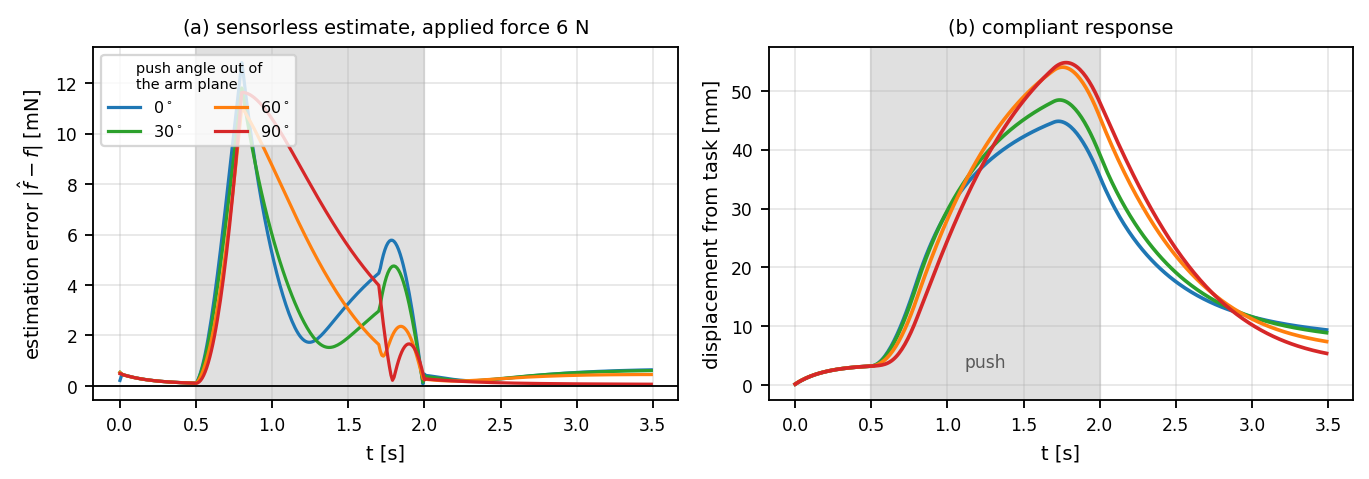
\includegraphics[width=0.92\textwidth]{interaction_traces.png}
\caption{Closed-loop interaction under a $6$~N push applied at four angles out of
the plane of the arm. (a) Error of the point-contact estimate. It stays below
$13$~mN, that is under $0.25\,\%$ of the applied force, at every angle including
the one the six-dimensional inversion cannot recover; the residual excursions
coincide with the ramps of the force profile and are the discretization floor of
the benchmark rather than a directional effect. (b) The resulting compliant
behavior: the arm yields by $45$ to $55$~mm under the push and returns towards the
task pose on release, at every angle. The directional dependence of the two
inversions is reported in Table~\ref{tab:threedirs}.}
\label{fig:traces}
\end{figure*}

Table~\ref{tab:mil} and Fig.~\ref{fig:traces} report the outcome. For the in-plane
push both estimators are accurate, which is the regime in which the conventional
inversion has historically been validated. For the normal push the
six-dimensional inversion is wrong by $83.4\,\%$ while the point-contact inversion
remains exact to the discretization floor of the benchmark. In both cases the
compliant loop yields under the push and returns on release, with the solver
reporting success at all $350$ steps.

Table~\ref{tab:threedirs} states the same result without reference to any angle,
for three directions that name themselves, at four configurations. A push along
the arm or along the base axis lies in the plane of the arm and both inversions
recover it. A push normal to that plane is recovered in full by the point-contact
inversion and largely converted into a moment by the six-dimensional one, at every
configuration tested.

\begin{table}[!t]
\caption{Recovered force for three physically named push directions, as a
percentage of the applied magnitude. The point-contact inversion returns
$100.0\,\%$ in every entry of the table.}
\label{tab:threedirs}
\centering
\footnotesize
\setlength{\tabcolsep}{4pt}
\begin{tabular}{lcccc}
\toprule
& \multicolumn{3}{c}{six-dimensional inversion [\%]} & spurious moment\\
\cmidrule(lr){2-4}
pose & along the arm & vertical & out of plane & out of plane\\
\midrule
P1 & $99.9$ & $100.0$ & $\bm{6.8}$  & $0.20$\\
P2 & $98.5$ & $100.0$ & $\bm{17.3}$ & $0.06$\\
P3 & $99.8$ & $100.0$ & $\bm{6.7}$  & $0.18$\\
P4 & $97.3$ & $100.0$ & $\bm{23.2}$ & $0.04$\\
\bottomrule
\end{tabular}
\vspace{2pt}
\\{\footnotesize \emph{along the arm}: radial direction of the end-effector;
\emph{vertical}: base axis; both lie in the plane of the arm.
\emph{out of plane}: normal to that plane. Moment in
$\mathrm{N}\cdot\mathrm{m}$ per newton applied.}
\end{table}

\subsection{Validation against an independent engine}
Replacing the analytic plant with MuJoCo and applying a known external force gives
a check that does not share the implementation of the dynamics. At the push peak
the applied force is $[0.00,\ 4.00,\ -1.50]$~N; the six-dimensional inversion
returns $[0.59,\ 0.23,\ -0.83]$~N and the point-contact inversion
$[0.21,\ 3.92,\ -1.31]$~N. Over the push window the RMSE against the applied force
falls from $2.227$~N to $0.157$~N, a factor of fourteen.

\begin{remark}[Interpretation of the residual error]
The remaining $0.157$~N is not estimator error, since the same estimator is exact
to $10^{-15}$ on the analytic plant. It is the model-to-engine gap: joint damping
and friction, the discrete constraint solver, and effects not represented in
\eqref{eq:dyn}. It is the best available proxy for hardware degradation and should
be read as a lower bound.
\end{remark}

\begin{remark}[Correlation is not accuracy]
In the same experiment the six-dimensional estimate correlates with ground truth
at $0.997$ while carrying the $2.227$~N error. That correlation measures
association rather than agreement, and is insensitive to gain and offset, is a
long-standing point in measurement comparison~\cite{bland1986agreement}; what the
experiment adds is that the failure mode is reached here by the estimator's own
structure rather than by noise, so a validation of this kind can appear healthy
while the quantity of interest is substantially wrong.
\end{remark}

\subsection{The compliant loop without a dynamic model}
\label{sec:res-model}
Section~\ref{sec:whichmodel} argued from a regulation test that the controller need
not carry a dynamic model. We repeat here the complete interaction loop of
Section~\ref{sec:res-estimation}, identical in every respect except that the
kinematic controller V0 replaces the torque-level controller T. The estimator is
unchanged and retains the dynamic model, which it requires.

\begin{table}[!t]
\caption{Complete compliant loop with a model-based controller (T) and a
model-free controller (V0). The estimator is identical in both.}
\label{tab:v0loop}
\centering
\footnotesize
\setlength{\tabcolsep}{4pt}
\begin{tabular}{llcccc}
\toprule
push & ctrl & force RMSE [N] & yield [mm] & return [mm] & ms/solve\\
\midrule
in plane & T  & $0.0299$ & $127.1$ & $11.23$ & $2.98$\\
         & V0 & $0.0332$ & $130.7$ & $\bm{9.24}$ & $\bm{0.119}$\\
\midrule
normal   & T  & $0.0042$ & $23.0$  & $3.71$  & $3.05$\\
         & V0 & $0.0045$ & $28.7$  & $\bm{1.92}$ & $\bm{0.123}$\\
\bottomrule
\end{tabular}
\end{table}

Table~\ref{tab:v0loop} reports the outcome. Force estimation is unaffected, as it
must be, since the estimator did not change. The compliant behavior is equivalent:
the arm yields comparably under the push and returns closer to the task pose on
release, in both push directions. The computational cost falls by a factor of
twenty-five. Carrying the inertia matrix and the bias term in the controller
therefore buys nothing on this platform, while carrying them in the estimator is
unavoidable.

\subsection{Robustness to servo noise}
\label{sec:res-noise}
Every result reported so far is noise-free, and on a clean bench an exact
estimator looks perfect by construction. We therefore evaluate both inversions
under the noise the MX-28R actually delivers: current quantization at
$3.36$~mA per count, Coulomb stiction of $0.05\,\mathrm{N}\cdot\mathrm{m}$ per
joint with random sign, which Section~\ref{sec:res-sens} identifies as the
dominant term, and twelve-bit encoder quantization.
Configurations are drawn uniformly over the joint ranges and contact forces
uniformly between $2$ and $10$~N, over $2000$ trials per condition.

\begin{table}[!t]
\caption{Monte Carlo under servo noise, $N=2000$. Relative force error, as a
percentage of the applied magnitude.}
\label{tab:noise}
\centering
\footnotesize
\setlength{\tabcolsep}{3.5pt}
\begin{tabular}{lcccccc}
\toprule
& \multicolumn{3}{c}{six-dimensional} & \multicolumn{3}{c}{point contact}\\
\cmidrule(lr){2-4}\cmidrule(lr){5-7}
noise & median & p90 & p99 & median & p90 & p99\\
\midrule
none          & $47.2$  & $86.8$  & $97.9$   & $\bm{0.0}$  & $\bm{0.0}$  & $\bm{0.0}$\\
nominal       & $69.6$  & $149.1$ & $1623$   & $\bm{18.0}$ & $\bm{58.9}$ & $\bm{353}$\\
$\times2$     & $89.3$  & $281.2$ & $3194$   & $\bm{35.9}$ & $\bm{118.3}$& $\bm{695}$\\
$\times4$     & $137.3$ & $548.4$ & $6239$   & $\bm{71.9}$ & $\bm{232.8}$& $\bm{1402}$\\
\bottomrule
\end{tabular}
\end{table}

Table~\ref{tab:noise} reports the outcome, and it is the honest expectation for
hardware. The point-contact inversion is no longer exact: its median relative
error is $18.0\,\%$ under nominal noise, against $69.6\,\%$ for the
six-dimensional one. The advantage is preserved at every percentile and under
degraded noise, but both distributions have heavy tails, which the conditioning
analysis of Section~\ref{sec:estimation} predicts and the next experiment
confirms.

\begin{table}[!t]
\caption{Effect of rejecting ill-conditioned postures, nominal noise.}
\label{tab:gating}
\centering
\footnotesize
\setlength{\tabcolsep}{5pt}
\begin{tabular}{ccccc}
\toprule
& \multicolumn{2}{c}{six-dimensional} & \multicolumn{2}{c}{point contact}\\
\cmidrule(lr){2-3}\cmidrule(lr){4-5}
$\sigma_{\min}(\Jv)$ threshold & median & p90 & median & p90\\
\midrule
$0.00$ & $69.6$ & $142.4$ & $18.0$ & $61.3$\\
$0.02$ & $70.8$ & $156.2$ & $16.2$ & $42.5$\\
$0.04$ & $69.0$ & $146.0$ & $14.5$ & $36.2$\\
$0.06$ & $77.7$ & $227.8$ & $\bm{12.4}$ & $\bm{29.5}$\\
\bottomrule
\end{tabular}
\end{table}

Table~\ref{tab:gating} discriminates between the two error mechanisms. Rejecting
postures below a threshold on $\sigma_{\min}(\Jv)$ halves the ninetieth percentile
of the point-contact estimator, from $61\,\%$ to $30\,\%$, exactly as
\eqref{eq:noise} predicts for an error that is amplified measurement noise. It
does nothing for the six-dimensional inversion, whose error is not noise but
structural misattribution and therefore cannot be gated away. The two mechanisms
identified analytically in Section~\ref{sec:estimation} are thus separable
experimentally, and monitoring $\sigma_{\min}(\Jv)$ online becomes an actionable
recommendation with a measured benefit.

\subsection{Direct verification of the conditioning bound}
\label{sec:res-cond}
Section~\ref{sec:res-noise} showed that rejecting ill-conditioned postures
shortens the tail of the point-contact estimator, which is consistent with
\eqref{eq:noise} but does not measure its exponent. We test the bound directly and
through the independent plant.

The arm is held at four postures spanning $\sigma_{\min}(\Jv)$ from $0.011$ to
$0.092$, a factor of nine, selected to be free of contact, clear of the floor, and
away from the joint limits. Sensor noise is injected on the current reading, which
is where the servo carries it, at one and at three quantization steps of the
MX-28R. For each posture we estimate the force sample by sample and record the
dispersion of the estimate, which is the quantity \eqref{eq:noise} bounds.

\begin{table}[!t]
\caption{Noise amplification through the MuJoCo plant. Dispersion of the
point-contact estimate at four postures, with sensor noise injected on the current
reading.}
\label{tab:condlaw}
\centering
\footnotesize
\setlength{\tabcolsep}{4pt}
\begin{tabular}{ccccc}
\toprule
$\sigma_{\min}(\Jv)$ & $\mathrm{std}(\bm\tau)$ & $\mathrm{std}(\hat{\bm f})$
& bound \eqref{eq:noise} & ratio\\
\midrule
\multicolumn{5}{l}{\emph{current noise $\sigma=3.4$~mA (one quantization step)}}\\
$0.0108$ & $0.0039$ & $0.183$ & $0.361$ & $0.51$\\
$0.0204$ & $0.0036$ & $0.096$ & $0.175$ & $0.55$\\
$0.0435$ & $0.0037$ & $0.044$ & $0.085$ & $0.51$\\
$0.0918$ & $0.0035$ & $0.030$ & $0.038$ & $0.77$\\
\midrule
\multicolumn{5}{l}{\emph{current noise $\sigma=10$~mA (three quantization steps)}}\\
$0.0108$ & $0.0102$ & $0.451$ & $0.945$ & $0.48$\\
$0.0204$ & $0.0103$ & $0.250$ & $0.504$ & $0.50$\\
$0.0435$ & $0.0102$ & $0.128$ & $0.233$ & $0.55$\\
$0.0918$ & $0.0102$ & $0.085$ & $0.111$ & $0.76$\\
\bottomrule
\end{tabular}
\end{table}

Table~\ref{tab:condlaw} reports the outcome. Fitting
$\log\mathrm{std}(\hat{\bm f})$ against $\log\sigma_{\min}(\Jv)$ gives a slope of
$-0.872$ with $R^2=0.980$ at the lower noise level and $-0.790$ with $R^2=0.987$
at the higher one, against the predicted $-1$. The dispersion therefore scales
essentially inversely with $\sigma_{\min}(\Jv)$ across a ninefold range, at two
noise levels, and through a plant whose damping, armature, and dry friction are
absent from the estimator model.

Two details are worth stating. The measured dispersion is consistently below the
bound, at $0.48$ to $0.77$ of it, which is as it should be: \eqref{eq:noise} is an
upper bound attained only when the residual error aligns with the least
observable direction. And the fitted slope is slightly shallower than $-1$ for the
same reason, since the alignment varies with posture.

\begin{remark}
The noise here is modeled rather than measured: MuJoCo is deterministic, so at
equilibrium the actuator torque is exactly constant and quantization alone
produces zero variance. What this experiment establishes is that the bound governs
the estimator when it is driven through the full nonlinear plant, not merely in
the algebraic setting of Section~\ref{sec:estimation}. Replacing the modeled noise
with a real servo's is the remaining step, and it requires only a static
measurement with the actuators disabled.
\end{remark}

\subsection{Sensitivity to model and calibration error}
\label{sec:res-sens}
Section~\ref{sec:velocity} places the error budget on the current-to-torque
calibration, and Section~\ref{sec:res-noise} shows stiction dominating the noise.
Both statements can be made precise by perturbing the validated model one
parameter at a time and recording the spurious force the estimator then reports
under no contact, which is the quantity a deployment would have to distinguish
from a real interaction. Table~\ref{tab:faults} reports it at the worst of six
configurations selected by sweeping the workspace for maximum sensitivity.

\begin{table}[!t]
\caption{Spurious force reported under no contact when a single model or
calibration parameter is perturbed, at the most sensitive of six configurations.}
\label{tab:faults}
\centering
\footnotesize
\setlength{\tabcolsep}{5pt}
\begin{tabular}{lc}
\toprule
perturbation & spurious $\norm{\hat{\bm f}_{3}}$ [N]\\
\midrule
inverted torque sign            & $8.75$\\
torque constant $\times2$       & $4.38$\\
torque offset $0.05\,\mathrm{N}\cdot\mathrm{m}$ & $1.31$\\
stiction $0.05\,\mathrm{N}\cdot\mathrm{m}$      & $1.09$\\
torque constant $+20\,\%$       & $0.88$\\
torque offset $0.02\,\mathrm{N}\cdot\mathrm{m}$ & $0.52$\\
link 4 mass $+20\,\%$           & $0.50$\\
joint zero shifted $0.10$~rad   & $0.33$\\
\midrule
\multicolumn{2}{c}{\emph{acceptance threshold $0.3$~N}}\\
\midrule
link 3 mass $+20\,\%$           & $0.29$\\
torque constant $+5\,\%$        & $0.22$\\
joint zero shifted $0.05$~rad   & $0.17$\\
link 2 mass $+20\,\%$           & $0.04$\\
link 1 mass $+20\,\%$           & $0.00$\\
\bottomrule
\end{tabular}
\end{table}

Two features of Table~\ref{tab:faults} matter for deployment. Torque offsets
dominate: $0.02\,\mathrm{N}\cdot\mathrm{m}$ already produces $0.52$~N, whereas a
$20\,\%$ error in a link mass produces $0.50$~N and a $5\,\%$ error in the torque
constant only $0.22$~N. The asymmetry is geometric. A gravity error lies in the
well-conditioned directions of $\Jv$ and is largely absorbed by the least-squares
projection of \eqref{eq:threesol}, whereas an offset is not, which is why stiction
rather than mass modeling sets the floor. The estimate is also insensitive to the
mass of the first link, correctly so, since that link rotates about a vertical axis
and gravity exerts no torque about it.

A practical consequence follows for calibration. Because gravity torques on this
arm are of order $0.3\,\mathrm{N}\cdot\mathrm{m}$, a no-contact null test cannot
resolve the torque constant: a $5\,\%$ error in it produces $0.22$~N, below the
threshold and indistinguishable from the residual bias of a well-modeled arm. The constant must therefore be identified
under a known load rather than at rest.

\subsection{Compliance versus rigid behavior}
\label{sec:res-control}
Six guidance conditions, each a task pose and a guidance direction, were run twice
in MuJoCo, once compliant and once rigid. The design is paired, both arms visiting
the identical conditions, so the between-condition variance is common and cancels.
The paired differences favor the compliant arm in all six conditions,
$+1.15\pm0.64$~N in guidance force and $+14.4\pm8.0$~mm in following error,
giving $t=4.42$ and $t=4.43$ against a two-sided critical value of $2.571$ at five
degrees of freedom. The unpaired summaries, $3.82\pm0.49$~N against
$2.67\pm1.09$~N, have overlapping dispersions and would not support the claim at
$N=6$: the effect is real and the unpaired presentation discards the information
that establishes it. This confirms that the estimate closes a compliant loop; it
is not offered as evidence for either contribution.

\subsection{Tracking, regulation, and computation}
Regulating to a fixed pose from an initial error of $0.160$~m converges to
$1.65$~mm with success at all $250$ steps. On a slow screw trajectory the
controller achieves $6.82$~mm position RMSE (maximum $7.40$~mm) and $4.79^\circ$
orientation RMSE (maximum $6.35^\circ$). Solve times appear in
Table~\ref{tab:timing}; we give two runs of the identical build because a single
timing run is not a measurement, and they differ by $17\,\%$ in the mean and
$59\,\%$ in the maximum.

% =========================================================================
\section{Discussion}
\label{sec:discussion}
% =========================================================================

\subsection{Practical implications}
The correction of Section~\ref{sec:estimation} is inexpensive to adopt. It
replaces one linear solve with another of smaller dimension and requires no
additional sensing, calibration, or tuning. For any application in which the
contact location is known by construction, and hand guiding at the end-effector is
the archetype, the six-dimensional inversion should not be used on an arm with
fewer than six joints.

The analysis also reframes the platform. A four-joint arm sensing contact force
through its own actuators is not operating at the margin of feasibility: by
Proposition~\ref{prop:exact} it has one measurement more than the problem
requires. The quantity a designer should examine when placing a task is
$\sigma_{\min}(\Jv)$, mapped in Fig.~\ref{fig:map}(b), not any index derived from
the rank deficit of the full Jacobian. Velocity-level actuation, in turn, removes
the need to identify the servo loop and renders the acceleration term negligible,
concentrating the design effort on a single calibration.

\subsection{Limitations}
\emph{Simulation only.} Every number reported here is obtained in simulation. The
model is exact against MuJoCo to $10^{-10}$ and MuJoCo serves as an independent
plant, but neither substitutes for the physical arm. Two quantities are expected
to degrade on hardware: the actuator-torque proxy from servo current, which
carries stiction and gearbox losses absent from \eqref{eq:dyn}, and the
finite-differenced acceleration, which will be noisier, although
Section~\ref{sec:velocity} shows the latter matters little. The $0.157$~N
model-to-engine gap is the best available proxy and is a lower bound.

\emph{Known contact point.} As stated in Remark~\ref{rem:cost}, the point-contact
model requires the contact location. Contact along the links, or contact
transmitting a moment through a grasped object, lies outside the analysis.

\emph{Conditioning near singularities.} Although $\mathrm{rank}\,\Jv=3$ throughout
the sampled workspace, $\sigma_{\min}(\Jv)$ reaches $7.6\times10^{-5}$, where
\eqref{eq:noise} predicts severe amplification. A deployment should monitor
$\sigma_{\min}(\Jv)$ online, which is inexpensive, and either avoid those postures
or widen the admittance dead band there.

\emph{Friction is not observed by either route.} The servo current measures motor
torque upstream of the gearbox, so gearbox friction is unmodeled whether the
applied torque is read from current or inferred from the velocity loop. This sets
the irreducible floor and is the quantity most likely to dominate on hardware.

\emph{Statistical scope.} The compliance result rests on six paired conditions in a
single simulator, and the timing figures vary by $17\,\%$ between two runs of an
identical build. We report both rather than the more favorable one.

\subsection{The experiment that would settle it}
\label{sec:protocol}
Two of the claims above are falsifiable on the physical arm at negligible cost,
and neither requires a force/torque sensor, a control loop, or a fast bus. The arm
is held with actuator torque disabled and positioned by hand at the four postures
of Fig.~\ref{fig:map}(b), spanning a factor of nine in $\sigma_{\min}(\Jv)$.

The first measures amplification. With nothing applied, the sample-to-sample
dispersion of $\hat{\bm f}_3$ is recorded at each posture; \eqref{eq:noise}
predicts that $\log\,\mathrm{std}\,\hat{\bm f}_3$ regresses on
$\log\,\sigma_{\min}(\Jv)$ with unit negative slope. A slope near zero refutes
Section~\ref{sec:conditioning}. This part cannot be rehearsed in simulation, since
a deterministic engine has no dispersion to measure.

The second measures accuracy and, more importantly, misattribution. A known load
is applied at the end-effector and both inversions are evaluated on the same
residual. A hanging mass supplies a vertical force and a luggage scale supplies a
horizontal one; two directions are required because a vertical force exerts no
moment about the vertical base axis and would leave that joint unexcited. The
prediction of Proposition~\ref{prop:split} is that the six-dimensional inversion
returns a nonzero moment where the true one is zero, and the outcome that would
refute this paper is the two inversions agreeing. The comparison is differential,
so the two measurements must share a Jacobian: if the arm sags under the load, the
posture change contaminates the difference and the test returns no verdict.

% =========================================================================
\section{Conclusion}
\label{sec:conclusion}
% =========================================================================

That a residual observer cannot resolve a full wrench from fewer than six joints,
and that a point-contact model reduces the unknown to three dimensions, is
established. This paper turns that statement into quantities a designer can use.
The force block of the wrench projector predicts where the six-dimensional
inversion fails and by how much: the loss is a linear function of the alignment
with the least observable direction at correlation $0.9993$ over $12\,000$
directions, and over $2197$ configurations it discards $50.5\,\%$ of an applied
unit force on average and up to $99.6\,\%$. That failure is silent, coexisting
with a $0.997$ correlation against ground truth, so a validation of the usual kind
does not detect it. In the noise-free model the point-contact inversion recovers
the force whenever $\mathrm{rank}\,\Jv=3$, which holds throughout the sampled
workspace, which leaves numerical conditioning as the binding limitation and makes
$\sigma_{\min}(\Jv)$ the quantity to monitor. Against an independent physics
engine the correction improves force RMSE by a factor of fourteen.

Velocity-level actuation, commonly regarded as an obstacle to sensorless
estimation, is instead a simplification. The servo reports the torque it applies,
so the residual is invariant to the inner loop and no identification of it is
required; the finite-differenced acceleration carries $0.006\,\%$ of the signal
and becomes irrelevant; and a kinematic controller matches a model-based one
throughout the compliant loop at one twenty-fifth of the cost, which confines the
dynamic model to the estimator. Under realistic servo quantization and stiction
the corrected estimator attains $18.0\,\%$ median relative error against
$69.6\,\%$, and gating on $\sigma_{\min}(\Jv)$ halves its tail while leaving the
six-dimensional error untouched, separating amplified noise from structural
misattribution. Finally, because the actuator saturates below the force range of
manual guidance, physical compliance is obtained for free and the synthetic loop
need only cover fine guidance and the return to task.

Two lines follow. The first is the hardware experiment of
Section~\ref{sec:protocol}, which tests the directional prediction, the
conditioning law, and the viability of inferring applied torque from servo
current, using a hanging mass and a luggage scale. Until it is run, the accuracy
figures reported here stand as model-based predictions and the estimator has not
been shown to survive gearbox friction, stiction, backlash, or the calibration of
the torque constant. The second is extending the contact model to an unknown
contact location along the links, which would restore whole-arm interaction while
preserving the dimensional argument that makes the approach work.

\bibliographystyle{IEEEtran}
\bibliography{refs}

% ⚠️ CAMARA LISTA: reemplazar IEEEbiographynophoto por IEEEbiography con la foto,
%    \begin{IEEEbiography}[{\includegraphics[width=1in,height=1.25in,clip,
%    keepaspectratio]{Fig/<nombre>.png}}]{Nombre}
%    No hay fotos en el repositorio, por eso van sin foto: asi compila.
\begin{IEEEbiographynophoto}{Bryan S. Guevara}
graduated in Mechatronic Engineering from the University of the Armed Forces ESPE
in 2018. In 2024 he earned his master's degree in Control Systems Engineering from
the National University of San Juan, where he also received the Ph.D. degree in
Control Systems Engineering. His research interests include robotics, dynamic
systems modeling, and optimal control.
\end{IEEEbiographynophoto}

\EOD

\vfill

\end{document}
